\documentclass{article}

\usepackage{scml2026}

\usepackage{multicol}
\usepackage[utf8]{inputenc} % allow utf-8 input
\usepackage[T1]{fontenc}    % use 8-bit T1 fonts
\usepackage{hyperref}       % hyperlinks
\usepackage{url}            % simple URL typesetting
\usepackage{booktabs}       % professional-quality tables
\usepackage{amsfonts}       % blackboard math symbols
\usepackage{amsmath}
\usepackage{amssymb}
\usepackage{nicefrac}       % compact symbols for 1/2, etc.
\usepackage{microtype}      % microtypography
\usepackage{cleveref}       % smart cross-referencing
\usepackage{graphicx}
\usepackage{natbib}
\usepackage{doi}
\usepackage{wrapfig}
\usepackage{float}

\title{Cluster-Weighted Extended Dynamic Mode Decomposition}
% Please provide a shortened title for the header
\renewcommand{\shorttitle}{CW-EDMD}

% Here you can change the date presented in the paper title
%\date{\today}
% Or remove it
\date{}

\author{%
	Lorenzo Tomaz\thanks{Corresponding author.} \\
	AE Studio \\
	\texttt{lorenzo.tomaz@ae.studio}
	\And
	Judd Rosenblatt \\
	AE Studio \\
	\texttt{judd@ae.studio}
	\And
	Flavio Kicis \\
	AE Studio \\
	\texttt{flavio.kicis@ae.studio}
	\And
	Thomas Berry Jones \\
	AE Studio \\
	\texttt{thomas@ae.studio}
	\And
	Diogo Schwerz de Lucena \\
	AE Studio \\
	\texttt{diogo@ae.studio}
}

%%% Add PDF metadata to help others organize their library
%%% Once the PDF is generated, you can check the metadata with
%%% $ pdfinfo paper.pdf
\hypersetup{
pdftitle={Cluster-Weighted Extended Dynamic Mode Decomposition},
pdfsubject={SCML2026 Abstract},
pdfauthor={Lorenzo Tomaz, Judd Rosenblatt, Flavio Kicis, Thomas Berry Jones, Diogo Schwerz de Lucena},
pdfkeywords={Koopman operator, EDMD, cluster-weighted models, EM, dynamical systems},
}

\begin{document}
\maketitle

\keywords{Koopman operator \and Extended Dynamic Mode Decomposition \and cluster-weighted models \and dynamical systems}

\begin{multicols}{2}

% =====================================================================
% §1 Lead paragraph
% =====================================================================
Extended Dynamic Mode Decomposition (EDMD) is the canonical data-driven approximation of the Koopman operator~\citep{williams2015edmd,mezic2005spectral,brunton2022modern,korda2018mpc,mauroy2020koopman}. Prior partitioning approaches predefine the partition by basin label~\citep{williams2015edmd}, phase-space stitching~\citep{sinha2020phase}, or operating-regime indicator~\citep{peitz2019switched}. We introduce \emph{Cluster-Weighted EDMD} (CW-EDMD), which learns the partition jointly with per-cluster operators via Expectation-Maximization (EM) on a cluster-weighted-model joint density~\citep{gershenfeld1999nature,ingrassia2014linear,punzo2014polynomial}, with responsibilities combining geometric proximity and per-cluster prediction residual. Across three classical systems (36 configurations, 10 seeds), CW-EDMD improves over EDMD at the matched polynomial lift degree, including the polynomial-exact degree of polynomial-RHS systems.

% =====================================================================
% §2 Method
% =====================================================================
\section{Method}
CW-EDMD is a Cluster-Weighted Model joint density $p(x_t,x_{t+1}) = \sum_{k=1}^{K} \pi_k\, \mathcal{N}(x_t; c_k, \Sigma_k)\, \mathcal{N}(\Delta x_k; 0, \sigma_k^2 I)$ with per-cluster prediction residual $\Delta x_k = x_{t+1} - c_k - [K_k\,\Phi(x_t-c_k)]_{1:d}$, where $\Phi$ is a degree-$q$ monomial lift centered at $c_k$ and $K_k$ is the per-cluster Koopman matrix. EM alternates between updating cluster responsibilities $r_{ik}\propto\pi_k\mathcal{N}(x_t;c_k,\Sigma_k)\mathcal{N}(\Delta x_k;0,\sigma_k^2 I)$, which combine geometric proximity with per-cluster prediction residual, and solving each $K_k$ in closed form by responsibility-weighted least squares, generalizing EDMD to the per-cluster regime (full derivation in Appendix~A).

\textbf{Experimental setup.} Three classical systems: Lorenz ($d{=}3$, polynomial-RHS deg-3), damped pendulum ($d{=}2$, non-polynomial $\sin\theta$), double-well Duffing ($d{=}2$, polynomial-RHS deg-3). Each: 12 configurations sweeping five sampling distributions, data size, domain, integrator step, and fit budget; 10 fixed seeds per configuration (full setup in Appendix~C; code and corpus in Appendix~F). We test \emph{matched-degree} CW-EDMD-$q$ against EDMD-$q$ via paired $t$-tests; a \emph{cross-config win} is \textit{p}\,$<\,0.05$ with lower CW-EDMD mean.

% =====================================================================
% §2 Results
% =====================================================================
\section{Results}
\textbf{Duffing oscillator (polynomial-RHS, degree 3).} CW-EDMD outperforms EDMD on all twelve configurations at three matched polynomial degrees ($q\in\{3,4,5\}$), with paired $t$-test \textit{p}\,$<\,10^{-4}$ throughout. At polynomial-exact $q{=}3$ (the conventional analytical floor), one-step error decreases $6.6{\times}10^{-5}\!\to\!2.4{\times}10^{-5}$, and at $q{=}5$ partitioning yields a further 1.6-fold reduction (Pareto frontier in Figure~\ref{fig:pareto-duffing}; per-system tables in Appendix~D). Damped pendulum (all twelve configurations, Figure~\ref{fig:pareto-pendulum}) and Lorenz (ten of twelve, Figure~\ref{fig:pareto-lorenz}; remaining two configurations characterized by the capacity-vs-data condition of Appendix~B) results appear in Appendix~D. \emph{Residual-aware partitioning thus improves over EDMD even at the polynomial-exact lift degree.}

\section*{Acknowledgments}
This work was conducted at AE Studio. The authors thank colleagues at AE Studio for discussions and feedback during the development of this work.

\bibliographystyle{plainnat}
\bibliography{references}

\end{multicols}

% =====================================================================
% Appendix (single-column for readable tables and equations)
% =====================================================================
\raggedbottom

\section*{Appendix A: Full Method Derivation}

\paragraph{Related work and positioning.} The idea of partitioning phase space and fitting a separate Koopman operator per region is not new. The original EDMD paper~\citep{williams2015edmd} demonstrates a partitioned EDMD on the Duffing oscillator by splitting the data along the basin-of-attraction boundary at $x{=}0$ and fitting separate operators to each basin, an early observation that per-region operators on dynamically meaningful partitions can outperform a single Koopman operator on the full phase space. Sinha, Nandanoori, and Yeung~\citep{sinha2020phase} formalize phase-space stitching of region-specific Koopman operators for large-scale dynamical systems. Peitz and Klus~\citep{peitz2019switched} develop a switched/multi-model Koopman formulation in which different operating regimes are assigned distinct linear Koopman models, with regime indicators driving the switch. Earlier mixture-of-experts work in the statistics literature~\citep{jordan1994hme,gershenfeld1999nature,ingrassia2014linear,punzo2014polynomial} provides the joint-density EM machinery that CW-EDMD reuses. The contribution of CW-EDMD relative to these works is the combination of three elements: (i) the partition is \emph{learned jointly} with the per-cluster operators by EM rather than predefined by basin label, geometry, or operating-regime indicator; (ii) the responsibilities used in the expectation step combine geometric proximity with per-cluster prediction residual, so that the partition tracks where each operator predicts well rather than where data is geometrically dense; and (iii) the per-cluster predictor is the discrete EDMD operator on a recentered polynomial lift, giving a clean apples-to-apples baseline of CW-EDMD against EDMD at matched lift degree. The geometry-only ablation in Appendix~E shows, on Duffing, that element (ii) is what drives the matched-degree advantage.

\paragraph{CWM joint density.} Given paired training data $\{(x_t^{(i)}, x_{t+1}^{(i)})\}_{i=1}^{N}$ in $\mathbb{R}^d$, we model the joint density as
\[
p(x_t, x_{t+1}) = \sum_{k=1}^{K} \pi_k\, p_X(x_t \mid k)\, p_{Y\mid X}(x_{t+1} \mid x_t, k),
\]
where $p_X(\cdot \mid k) = \mathcal{N}(c_k, \Sigma_k)$ is the cluster's geometric component and $p_{Y\mid X}(\cdot \mid x_t, k) = \mathcal{N}(\hat{x}_{t+1\mid k}, \sigma_k^2 I)$ is the per-cluster prediction. Mixture weights $\pi_k$ satisfy $\sum_k \pi_k = 1$. Compared with a Gaussian mixture model (GMM), the second factor introduces \emph{residual awareness}: cluster $k$ takes responsibility only for points it can predict well, not just points geometrically nearby.

\paragraph{Per-cluster Koopman operator.} For each cluster $k$ with center $c_k$, define the recentered monomial lift $\Phi: \mathbb{R}^d \to \mathbb{R}^{M_q}$ of total degree $\leq q$, where $M_q = \binom{d+q}{q}$. The per-cluster prediction is
\[
\hat{x}_{t+1\mid k} = c_k + [K_k\, \Phi(x_t - c_k)]_{1:d},
\]
where $K_k \in \mathbb{R}^{M_q \times M_q}$ is the Koopman matrix and the projection $[\cdot]_{1:d}$ recovers the state. We retain the full square $K_k$ rather than a rectangular $\mathbb{R}^{d\times M_q}$ regression onto the state because the square form is the standard EDMD discretization of the Koopman operator on the lifted observable space~\citep{williams2015edmd,brunton2022modern}: it preserves the full lifted-space spectrum and lets the operator be reused for spectral analyses, eigenfunction extraction, and downstream control. The output projection is applied only at prediction time, not at fit time. The cost is the $M_q^2 - d\,M_q$ unused parameters per cluster; we report this overhead in the parameter counts of all tables.

\paragraph{EM updates.} Let $r_{ik}$ be the posterior responsibility of cluster $k$ for sample $i$. The expectation step (responsibility update) is
\[
r_{ik} \propto \pi_k\, \mathcal{N}(x_t^{(i)}; c_k, \Sigma_k)\, \mathcal{N}\!\bigl(x_{t+1}^{(i)} - \hat{x}_{t+1\mid k}^{(i)}; 0, \sigma_k^2 I\bigr),
\]
combining geometric proximity (first Gaussian) with prediction residual (second Gaussian). The maximization step (parameter update) then updates each cluster:
\[
c_k = \frac{\sum_i r_{ik} x_t^{(i)}}{\sum_i r_{ik}}, \quad
\Sigma_k = \frac{\sum_i r_{ik} (x_t^{(i)}-c_k)(x_t^{(i)}-c_k)^\top}{\sum_i r_{ik}},
\]
\[
K_k = \arg\min_{K} \sum_i r_{ik}\,\bigl\| \Phi(x_{t+1}^{(i)} - c_k) - K\,\Phi(x_t^{(i)} - c_k) \bigr\|^2,
\]
which has the closed-form weighted-least-squares solution
\[
K_k = \bigl(\tilde{Y}_k W_k \tilde{X}_k^\top\bigr)\bigl(\tilde{X}_k W_k \tilde{X}_k^\top + \lambda I\bigr)^{-1},
\]
with $\tilde{X}_k, \tilde{Y}_k$ the lifted recentered training data, $W_k = \mathrm{diag}(r_{ik})$, and a small Tikhonov regularizer $\lambda$. Finally $\sigma_k^2$ is updated from the responsibility-weighted residual variance.

\paragraph{Empty-cluster pruning.} A weak Dirichlet prior $\mathrm{Dir}(\alpha)$ on $\boldsymbol{\pi}$ with $\alpha < 1$ allows components with vanishing responsibility to be pruned between iterations.

\paragraph{Initialization.} We initialize $c_k$ by $K$-means and $K_k$ by ordinary EDMD on the points initially assigned to cluster $k$. EM is run with multiple restarts and the highest-likelihood run is retained.

\paragraph{Rollout.} At inference, given current state $x_t$, the rollout cluster index is $k^*(x_t) = \arg\max_k\, \pi_k\, \mathcal{N}(x_t; c_k, \Sigma_k)$ (geometry-only at test time, since no $x_{t+1}$ is available), and the next state is $x_{t+1} = c_{k^*} + [K_{k^*} \Phi(x_t - c_{k^*})]_{1:d}$. Multi-step rollouts iterate this map. \emph{No derivatives, no Euler step.}

\section*{Appendix B: Capacity-vs-Data Operating Regime}

Each cluster's Koopman operator $K_k \in \mathbb{R}^{M_q \times M_q}$ has $M_q^2$ free parameters, with $M_q = \binom{d+q}{q}$. EM with $K$ clusters distributes the $N$ training pairs across components, giving roughly $P/K$ samples per cluster after responsibility assignment, where $P$ is the count of \emph{decorrelated} training samples. Under the classical regression-underdetermination heuristic that parameter count should not exceed roughly half the sample count, this motivates the candidate condition
\[
K \cdot M_q^2 \le \tfrac{1}{2}\,P_{\text{eff}}.
\]

\paragraph{Post-hoc nature of the rule.} We are explicit that this condition is \emph{post-hoc}: it was derived after observing the two Lorenz non-wins, by asking what those configurations had in common. It is not a prospective prediction validated against held-out failures. The rule has tunable degrees of freedom (the one-half safety factor; the choice of timescale $\tau$ entering $P_{\text{eff}}$; and the choice of $P_{\text{eff}} \approx N\,\Delta t/\tau$ as the proxy for decorrelated sample count, in the absence of a closed-form expression for chaotic dynamics), so a fit between the rule and the observed failures is necessary but not sufficient evidence for predictive validity. What we report is consistency: the two Lorenz non-wins occur in regimes where $K M_q^2$ approaches or exceeds $P_{\text{eff}}$, while the ten winning Lorenz regimes have $P_{\text{eff}}$ several times larger than $K M_q^2$, and damped pendulum and Duffing (smaller $M_q$, denser data) are uniformly well below the underdetermination threshold. Prospective validation, on a new system where the rule predicts a failure that is then observed, is the natural next test; more principled estimators of $P_{\text{eff}}$ based on autocorrelation length or block-bootstrap effective sample size would also tighten the rule.
For Lorenz at $q{=}3$, $M_q^2 = 400$. With $N{=}500$ and $K{=}12$, one has $K\cdot M_q^2 = 4800 \gg 250$, an order-of-magnitude violation: this is the small-training-data Lorenz attractor configuration. With $\Delta t=0.005$ on the chaotic Lorenz attractor, $P_{\text{eff}}$ at $N{=}2000$ collapses far below $2000$ due to high temporal correlation between consecutive states, again violating the rule: this is the short-integrator-step Lorenz configuration. All 10 winning Lorenz configurations satisfy $P_{\text{eff}} \geq 4 M_q^2$ comfortably. The rule is restrictive but predictive: it tells the practitioner when partitioning is worth the parameter cost, and is the principal methodological constraint we report.

\section*{Appendix C: Full Experimental Setup}

\paragraph{Systems.} The three classical systems used in this work, all expressed as continuous-time autonomous ODEs and then integrated to produce discrete-time pairs $(x_t, x_{t+1})$ at fixed step $\Delta t$:

\emph{Lorenz attractor} ($d=3$, polynomial RHS of degree 3):
\[
\dot{x} = \sigma(y - x), \quad
\dot{y} = x(\rho - z) - y, \quad
\dot{z} = x y - \beta z,
\]
with parameters $(\sigma, \rho, \beta) = (10, 28, 8/3)$. The attractor exhibits strange-attractor chaos with two folding wings around the unstable origin.

\emph{Damped pendulum} ($d=2$, non-polynomial RHS):
\[
\dot{\theta} = \omega, \qquad
\dot{\omega} = -\sin\theta - \gamma\, \omega,
\]
with damping coefficient $\gamma = 0.1$. The non-polynomial $\sin\theta$ term is the reason no global polynomial lift is exact at any finite degree; this is the system on which the parameter-efficiency advantage of CW-EDMD is largest.

\emph{Double-well Duffing oscillator} ($d=2$, polynomial RHS of degree 3):
\[
\dot{x} = v, \qquad
\dot{v} = x - x^3 - \delta\, v,
\]
with damping $\delta = 0.2$. The cubic restoring force $x - x^3$ creates two stable foci at $x = \pm 1$ and an unstable saddle at $x = 0$. The polynomial-exact lift degree is $q = 3$; this is the system in which CW-EDMD wins at the analytical floor.

\paragraph{Discretization.} All systems are integrated with vectorized RK4. Pair generation produces $(x_t, x_{t+1})$ at fixed step $\Delta t$, with $\Delta t \in \{0.005, 0.01, 0.05, 0.1\}$ across configurations.

\paragraph{Sampling distributions.} Five distributions are swept independently per system: \emph{uniform} over a configurable box, \emph{Gaussian} centered at the origin, \emph{Gaussian mixture} centered at attractor foci, \emph{periodic-noise} (sinusoidal with additive noise), and \emph{trajectory ensemble} (random ICs integrated for several steps, all trajectory points used as training). Additional Lorenz-specific \emph{single-trajectory attractor} sampling is used for two attractor-baseline configurations.

\paragraph{Configurations.} 12 configurations per system, each varying one factor relative to a baseline (data size, box size, $\Delta t$, fit budget, sampling distribution).

\paragraph{Seeds.} 10 fixed seeds per (system, configuration, method): $\{1, 42, 101, 307, 1001, 7789, 13245, 11, 103, 13\}$. Seeds control train/test sampling, EM initialization, and integrator noise.

\paragraph{Methods.} EDMD at degrees $\{2,3,4,5\}$ (Lorenz, damped pendulum, Duffing) and $\{6,8\}$ (damped pendulum only); CW-EDMD at degrees $\{2,3\}$ (Lorenz), $\{2,4\}$ (damped pendulum), $\{2,3,4,5\}$ (Duffing) with $K \in \{2,4,8,16\}$ where the capacity-vs-data rule permits.

\paragraph{Metrics.} (i)~\emph{One-step error}: mean $\ell_2$ prediction error on the held-out test set. (ii)~\emph{Rollout error at $H$ seconds}: mean $\ell_2$ error of the iterated map at horizons $H \in \{1,2,5,10,20\}$\,s, averaged over test initial conditions.

\paragraph{Statistics.} For each (system, configuration, metric) we run all methods over 10 seeds and compute mean and 95\% CI. \emph{Paired $t$-tests} (per-seed pairing) test the matched-degree comparison ``CW-EDMD $q$ vs.\ EDMD $q$''. A cross-configuration outcome is a \emph{win} if \textit{p}\,$<\,0.05$ and the CW-EDMD mean is lower; a \emph{loss} if \textit{p}\,$<\,0.05$ and higher; a \emph{tie} otherwise. We report wins / losses / ties tallied across the 12 configurations.

\section*{Appendix D: Per-System Detailed Results}

\begin{figure}[H]
	\begin{center}
		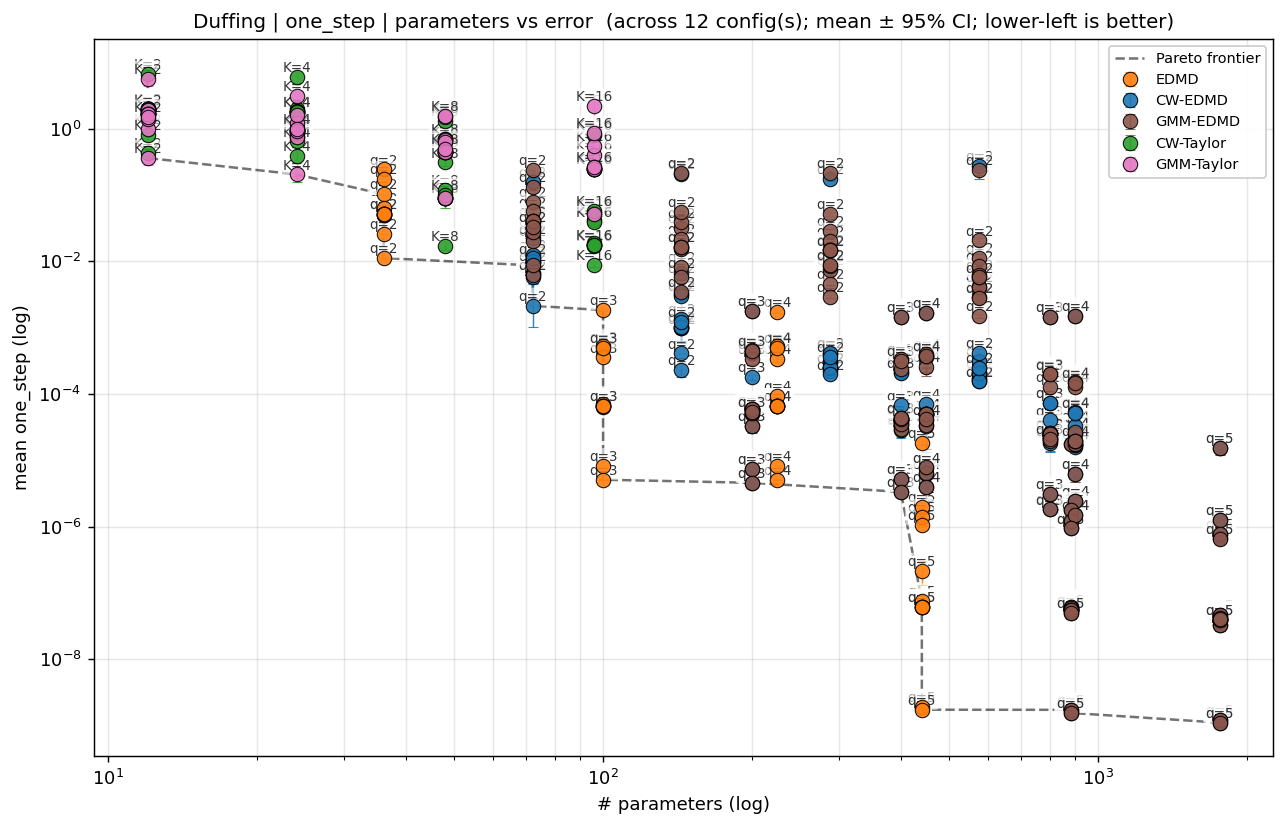
\includegraphics[width=0.85\textwidth]{pareto_duffing.png}
	\end{center}
	\caption{\textbf{Duffing Pareto frontier: median one-step error vs.\ parameter count.} Each point is one (method, hyperparameter) combination summarized across 12 configurations $\times$ 10 seeds. Blue: CW-EDMD (the focus of this paper). Orange: EDMD at increasing polynomial degree. Brown: GMM-EDMD (the within-EDMD ablation, with the residual-aware responsibility update replaced by GMM-style proximity-only responsibilities). Green: CW-Taylor (Appendix~E, the Taylor-predictor variant). Pink: GMM-Taylor (the within-Taylor ablation, the standard CWM contrast point of geometry-only responsibilities + per-cluster regression). Dashed: Pareto frontier. CW-EDMD dominates EDMD at the polynomial-exact degree ($q{=}3$) and at the over-exact degree ($q{=}5$, machine-precision regime).}
	\label{fig:pareto-duffing}
\end{figure}

\begin{figure}[H]
	\begin{center}
		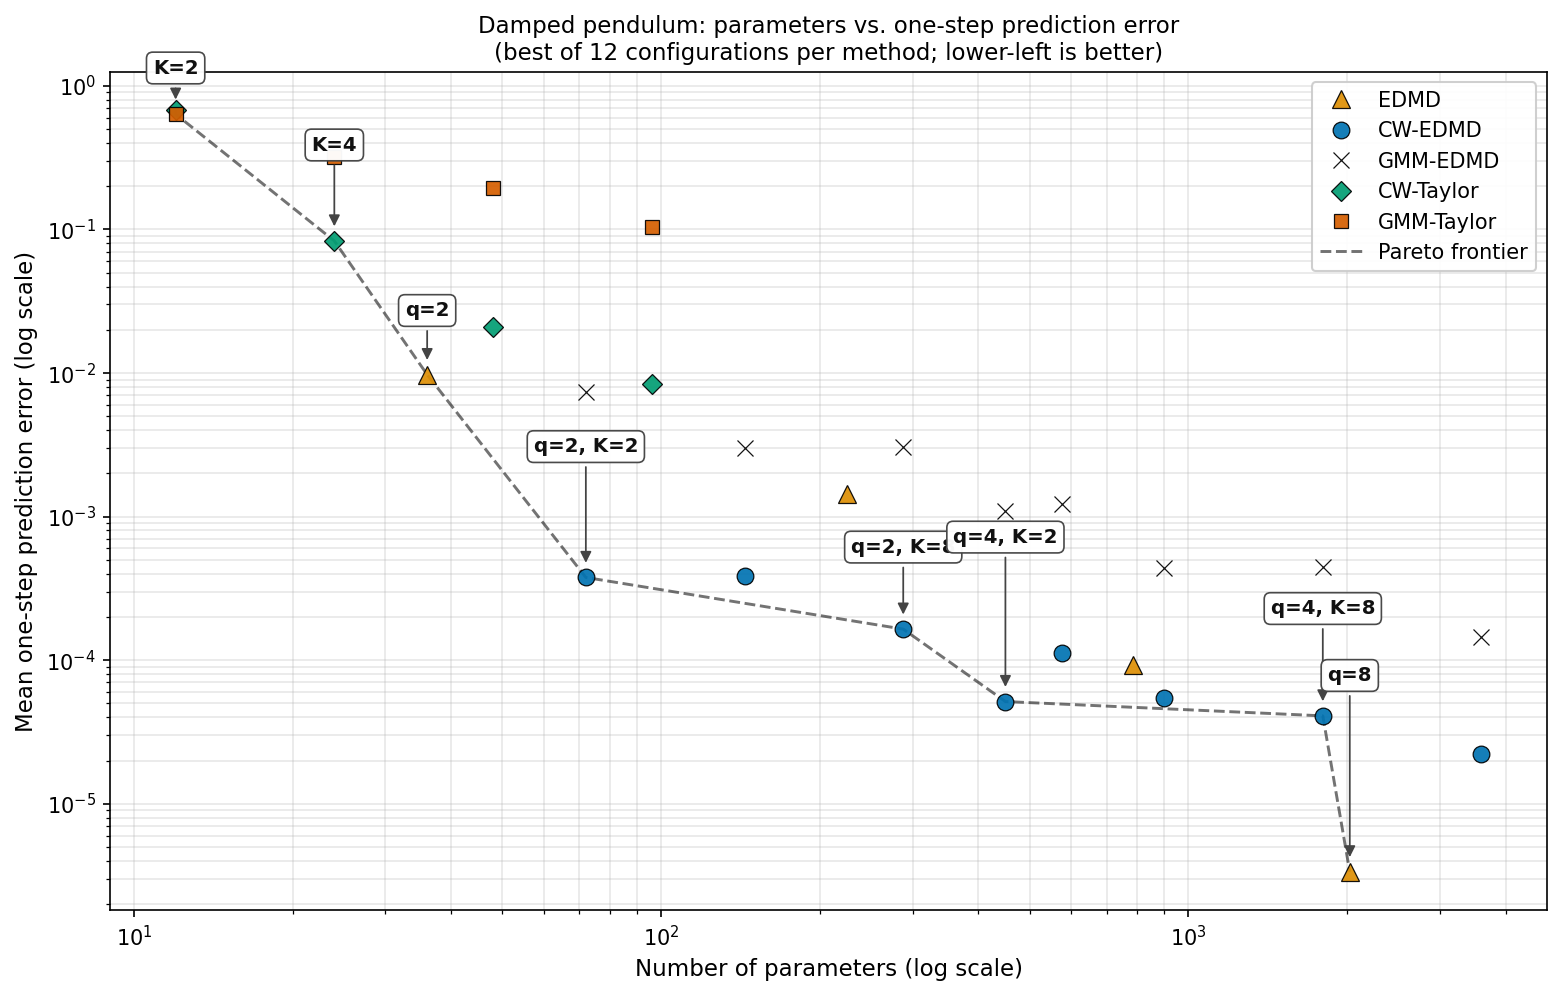
\includegraphics[width=0.85\textwidth]{pareto_pendulum.png}
	\end{center}
	\caption{\textbf{Damped pendulum Pareto frontier: median one-step error vs.\ parameter count.} Same conventions as Figure~\ref{fig:pareto-duffing}. Matched-degree CW-EDMD ($q{=}4$, blue stars at the bottom of the plot) strictly dominates all EDMD parameter budgets, including $q{=}8$ at 2025 parameters. Higher polynomial degrees overfit; partitioning does not.}
	\label{fig:pareto-pendulum}
\end{figure}

\begin{figure}[H]
	\begin{center}
		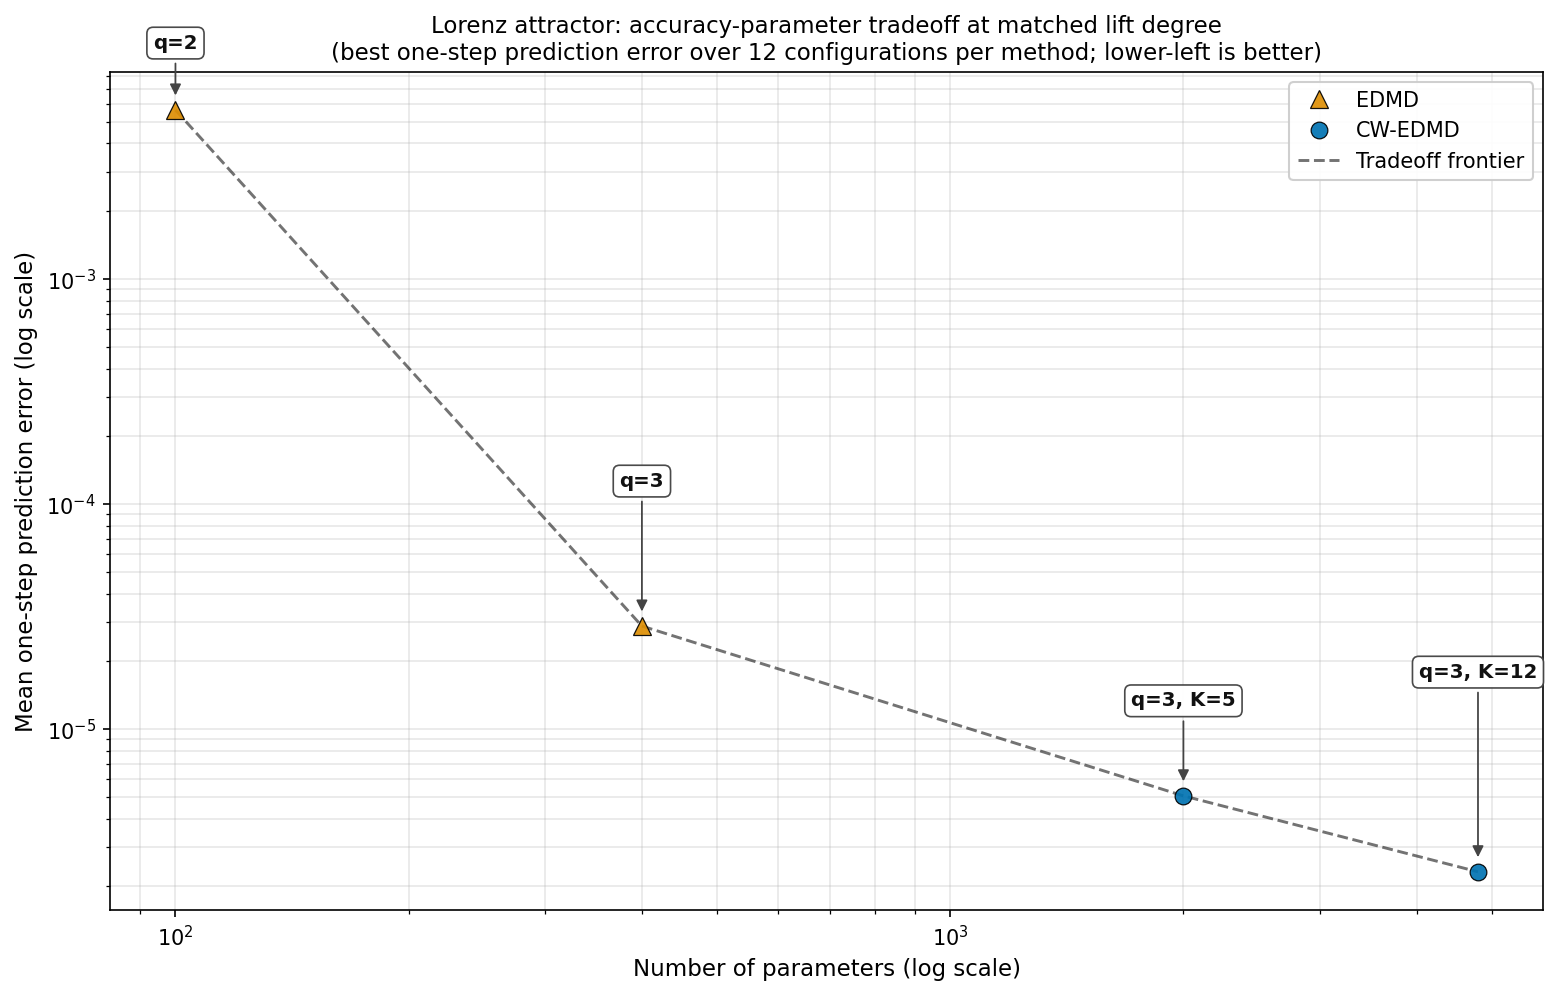
\includegraphics[width=0.85\textwidth]{pareto_lorenz.png}
	\end{center}
	\caption{\textbf{Lorenz Pareto frontier: median one-step error vs.\ parameter count.} Same conventions as Figure~\ref{fig:pareto-duffing}. CW-EDMD at the matched polynomial-exact degree ($q{=}3$) Pareto-dominates EDMD on the ten configurations satisfying the capacity-vs-data constraint of Appendix~B. The two non-winning configurations (small training data and short integrator step) are dominated by the operating-regime issue, not the partitioning principle.}
	\label{fig:pareto-lorenz}
\end{figure}

\paragraph{Damped pendulum.} At matched lift degree $q{=}4$, median prediction error in dimensionless state-space units across the 12 configurations and 10 seeds is reported in Table~\ref{tab:pendulum}. Median is reported in preference to mean because rollout error on a small subset of high-dynamic-range configurations diverges to large values that dominate the cross-configuration mean.
\begin{table}[H]
\caption{Damped pendulum at matched lift degree $q{=}4$: median prediction error (dimensionless state-space units) across 12 configurations and 10 seeds.}
\label{tab:pendulum}
\centering\small
\begin{tabular}{lrrrr}
\toprule
Method & Params & one-step & 5\,s & 10\,s \\
\midrule
EDMD $q{=}2$ & 36 & $8.0\!\times\!10^{-2}$ & $1.16\!\times\!10^{0}$ & $8.9\!\times\!10^{-1}$ \\
EDMD $q{=}4$ & 225 & $1.5\!\times\!10^{-1}$ & $2.7\!\times\!10^{0}$ & $2.8\!\times\!10^{0}$ \\
EDMD $q{=}8$ & 2025 & $1.8\!\times\!10^{-1}$ & $2.2\!\times\!10^{0}$ & $2.3\!\times\!10^{0}$ \\
CW-EDMD $q{=}4, K{=}4$ & 900 & $\mathbf{8.5\!\times\!10^{-5}}$ & $\mathbf{4.4\!\times\!10^{-3}}$ & $\mathbf{5.9\!\times\!10^{-3}}$ \\
CW-EDMD $q{=}4, K{=}8$ & 1800 & $\mathbf{5.1\!\times\!10^{-5}}$ & $\mathbf{2.1\!\times\!10^{-3}}$ & $\mathbf{3.1\!\times\!10^{-3}}$ \\
CW-EDMD $q{=}4, K{=}16$ & 3600 & $\mathbf{3.4\!\times\!10^{-5}}$ & $\mathbf{1.5\!\times\!10^{-3}}$ & $\mathbf{1.5\!\times\!10^{-3}}$ \\
\bottomrule
\end{tabular}
\end{table}
\noindent CW-EDMD $q{=}4, K{=}8$ wins on all twelve configurations against EDMD $q{=}4$ (paired mean difference $-2.80$ on 10\,s rollout) and against EDMD $q{=}8$ (paired mean difference $-2.28$).

\paragraph{Duffing.} At three matched polynomial degrees, median prediction error across the 12 configurations and 10 seeds is reported in Table~\ref{tab:duffing}, with EDMD baselines at every matched degree for direct comparison.
\begin{table}[H]
\caption{Duffing oscillator: median prediction error (dimensionless state-space units) across 12 configurations and 10 seeds. Top block: EDMD at four polynomial lift degrees. Bottom block: CW-EDMD at three matched lift degrees.}
\label{tab:duffing}
\centering\small
\begin{tabular}{lrrr}
\toprule
Method & Params & one-step & 10\,s \\
\midrule
EDMD $q{=}2$                    & 36   & $5.2\!\times\!10^{-2}$ & $9.1\!\times\!10^{-1}$ \\
EDMD $q{=}3$ (polynomial-exact) & 100  & $6.6\!\times\!10^{-5}$ & $7.0\!\times\!10^{-3}$ \\
EDMD $q{=}4$ (over-exact)       & 225  & $6.7\!\times\!10^{-5}$ & $7.0\!\times\!10^{-3}$ \\
EDMD $q{=}5$ (over-exact)       & 441  & $6.7\!\times\!10^{-8}$ & $5.1\!\times\!10^{-6}$ \\
\midrule
CW-EDMD $q{=}3, K{=}8$  & 800  & $\mathbf{2.4\!\times\!10^{-5}}$ & $\mathbf{2.0\!\times\!10^{-3}}$ \\
CW-EDMD $q{=}4, K{=}4$  & 900  & $\mathbf{1.9\!\times\!10^{-5}}$ & $\mathbf{8.1\!\times\!10^{-4}}$ \\
CW-EDMD $q{=}5, K{=}4$  & 1764 & $\mathbf{4.3\!\times\!10^{-8}}$ & $\mathbf{3.4\!\times\!10^{-6}}$ \\
\bottomrule
\end{tabular}
\end{table}
\noindent CW-EDMD wins on all twelve configurations at each of the three matched degrees against EDMD (\textit{p}\,$<\,10^{-4}$ in every configuration). The within-Taylor ablation against the standard GMM-clustered local model contrast point of the CWM literature is reported in Appendix~E.

\paragraph{Lorenz.} Median prediction error across the 12 configurations and 10 seeds is reported in Table~\ref{tab:lorenz}. The metric \emph{r5s} reaches the rollout-step cap on the chaotic configurations and saturates; \emph{one-step} is the cleanest cross-method comparison.
\begin{table}[H]
\caption{Lorenz attractor: median prediction error (dimensionless state-space units) across 12 configurations and 10 seeds. Top block: EDMD at two polynomial lift degrees. Middle block: CW-EDMD at lift degree $q{=}2$ (mismatched). Bottom block: CW-EDMD at the matched polynomial-exact degree $q{=}3$.}
\label{tab:lorenz}
\centering\small
\begin{tabular}{lrrr}
\toprule
Method & Params & one-step & 5\,s \\
\midrule
EDMD $q{=}2$                    & 100  & $2.0\!\times\!10^{-2}$ & $3.2\!\times\!10^{0}$ \\
EDMD $q{=}3$ (polynomial-exact) & 400  & $2.2\!\times\!10^{-4}$ & $4.5\!\times\!10^{-2}$ \\
\midrule
CW-EDMD $q{=}2, K{=}5$         & 500  & $2.2\!\times\!10^{-3}$ & $5.5\!\times\!10^{-1}$ \\
CW-EDMD $q{=}2, K{=}12$        & 1200 & $4.2\!\times\!10^{-4}$ & $1.0\!\times\!10^{-1}$ \\
CW-EDMD $q{=}2, K{=}20$        & 2000 & $2.5\!\times\!10^{-4}$ & $6.3\!\times\!10^{-2}$ \\
\midrule
CW-EDMD $q{=}3, K{=}5$         & 2000 & $\mathbf{2.5\!\times\!10^{-5}}$ & $\mathbf{2.8\!\times\!10^{-2}}$ \\
CW-EDMD $q{=}3, K{=}12$        & 4800 & $\mathbf{6.3\!\times\!10^{-6}}$ & $\mathbf{2.4\!\times\!10^{-2}}$ \\
CW-EDMD $q{=}3, K{=}20$        & 8000 & $\mathbf{5.8\!\times\!10^{-6}}$ & $\mathbf{2.9\!\times\!10^{-2}}$ \\
\bottomrule
\end{tabular}
\end{table}
\noindent At the matched polynomial-exact degree $q{=}3$, CW-EDMD with $K{=}12$ wins on ten of twelve configurations against EDMD $q{=}3$ (paired Wilcoxon \textit{p}\,$<\,0.05$, mean differences up to $-2.3\!\times\!10^{-4}$); the remaining two configurations correspond to capacity-vs-data violations described in Appendix~B (small training data and short integrator step). At fixed $K{=}5$ ($500$--$2000$ parameters), increasing the lift degree from $q{=}2$ to $q{=}3$ decreases one-step error by roughly two orders of magnitude, demonstrating that the matched lift degree is essential for the partitioning advantage on this polynomial-RHS system. The mismatched $q{=}2$ CW-EDMD entries are included for ablation.


\section*{Appendix E: Generality and Initialization}

\paragraph{CWM framing and approximator-agnostic per-cluster fit.} CW-EDMD instantiates the cluster-weighted-model framework~\citep{gershenfeld1999nature,ingrassia2014linear,punzo2014polynomial} with EDMD as the per-cluster predictor. The CWM joint density $p(x_t, x_{t+1}) = \sum_k \pi_k\, p_k(x_t)\, p_k(x_{t+1}\mid x_t)$ is agnostic in the per-cluster predictor $p_k(x_{t+1}\mid x_t)$. We provide a Taylor-expansion variant in our implementation that replaces the per-cluster EDMD operator with a first-order centered linearization $\hat{x}_{t+1\mid k} = c_k + (I + \Delta t\, J(c_k))(x_t - c_k)$ when an analytic Jacobian is available at cluster centers; the same EM machinery applies. This drop-in substitutability is what we mean by \emph{model-agnostic}: any local approximator that admits a fit-time loss and an inference-time prediction can be substituted. The headline matched-degree comparisons in the main text are restricted to EDMD by design, to make the partitioning hypothesis a clean controlled test on one approximator family.

\paragraph{Within-Taylor ablation against the GMM-clustered local model contrast.} The classical contrast point for CWM in the statistical-clustering literature~\citep{ingrassia2014linear} is the two-stage approach of GMM clustering followed by per-cluster regression --- a \emph{GMM-clustered local model} in which responsibilities depend only on geometric proximity to cluster centers, with no per-cluster prediction-quality factor. In our framework this corresponds to setting the residual variance $\sigma^2 \to \infty$ in the CWM responsibility update, which makes the per-cluster prediction-likelihood term flat and reduces the E-step to standard GMM. We run this ablation on the Taylor variant across all three systems (Lorenz, damped pendulum, Duffing) at matched cluster count $K$. The ablation reveals a $K$-dependent pattern.

At moderate-to-large cluster counts, the residual-aware responsibility update yields decisive gains over the GMM-clustered local model: on Duffing at $K{\geq}8$ (factors of $4.5$--$12.8\times$ in median one-step error, $10$--$11$ wins of $12$ configurations), on the damped pendulum at $K{\geq}4$ (factors of $3.2$--$11.5\times$, $8$--$12$ wins of $12$), and on Lorenz at all tested $K$ (factors of $1.6$--$4.1\times$, $12/12$ wins at every $K\in\{5,12,20,50\}$). At small cluster counts the picture inverts: on Duffing at $K\in\{2,4\}$ and on the damped pendulum at $K{=}2$, the two methods are statistically equivalent or the GMM-clustered baseline is slightly better (e.g., Duffing $K{=}2$: residual-aware median $1.98$ vs.\ GMM-clustered median $1.87$, paired Wilcoxon favoring the GMM-clustered baseline in $11/12$ configurations). The interpretation is intuitive: the residual-aware mechanism contributes when the partition has enough freedom to be ambiguous geometrically; with very few clusters, geometric proximity is already a near-unique cluster assignment and the prediction-residual factor adds noise rather than information.

\paragraph{Implication for CW-EDMD.} The within-Taylor ablation establishes that the residual-aware responsibility update is essential at the cluster counts where partitioning provides meaningful parameter freedom, across all three systems and the Taylor predictor family. CW-EDMD uses the same EM machinery with EDMD substituted for Taylor as the per-cluster predictor; by the model-agnostic substitutability of CWM, the same residual-aware mechanism is expected to drive the matched-degree advantage in the EDMD branch as well. A direct within-EDMD analogue of the within-Taylor ablation reported above --- i.e., a CW-EDMD variant whose responsibility update is replaced by the GMM-style proximity-only rule (the same $\sigma^2 \to \infty$ degeneration applied to the EDMD branch instead of the Taylor branch), compared at matched cluster count and lift degree against full CW-EDMD --- would close this inference by direct measurement and is the natural follow-up experiment.

\paragraph{Initialization.} We initialize $c_k$ by $K$-means and $K_k$ by ordinary EDMD on the points initially assigned to cluster $k$, with multi-restart EM. Multi-restart is essential on Duffing wide-box configurations where the cubic nonlinearity creates deep local minima.

\paragraph{Computational cost.} EDMD fits a single closed-form regression of size $M_q^2$ in one shot. CW-EDMD replaces this with $K$ regressions of the same size per EM iteration, with $T$ iterations and $R$ restarts, giving a fit cost of order $R \cdot T \cdot K \cdot M_q^2 \cdot N$ versus $M_q^2 \cdot N$ for EDMD. In the configurations reported here ($T \le 80$ iterations, $R \le 2$ restarts, $K \le 16$), the worst-case CW-EDMD fit is roughly $80 \cdot 2 \cdot 16 \approx 2.6\times10^3$ times the cost of a single EDMD fit. Inference cost is comparable to EDMD: rollout requires one $K_k\,\Phi(\cdot)$ matrix-vector product per step plus a Gaussian-likelihood evaluation to pick the active cluster.

\paragraph{Limitations.} Four limitations of the present study are worth flagging. First, the residual-aware vs.\ GMM-clustered ablation is run within the Taylor predictor family across all three systems; the corresponding direct within-EDMD analogue --- a CW-EDMD variant with its responsibility update replaced by the GMM-style proximity-only rule, compared against full CW-EDMD at matched cluster count and lift degree --- is not in the present corpus, and the implication for CW-EDMD is by analogy across the model-agnostic CWM machinery rather than direct measurement. Second, the operating-regime condition of Appendix~B is post-hoc: it was derived to be consistent with the two observed Lorenz non-wins, not pre-registered or validated on held-out failures, and the proxy $P_{\text{eff}} \approx N\,\Delta t/\tau$ has tunable degrees of freedom. The condition should be treated as a hypothesis to be tested prospectively on a new system where it predicts a failure that is then observed, rather than as a validated bound. Third, the Lorenz results are mixed (ten wins, two non-wins out of twelve configurations), and while the non-wins are characterizable in terms of capacity-vs-data, the absence of a clean win across all Lorenz configurations is a real limitation of the cross-system claim. Fourth, the corpus is restricted to autonomous low-dimensional systems with smooth dynamics; control-input-driven systems and higher-dimensional flows (where CW-EDMD's parameter count grows quadratically in $M_q$) are out of scope here.

\section*{Appendix F: Reproducibility}

All experimental configurations are versioned as YAML files dispatched through a single statistical-validation driver (\texttt{validation/run\_statistical.py --config <name>.yaml}). Per-seed JSON results are written for every (system, configuration, method, seed) combination and aggregated post-hoc into the long-form CSV used for the figures and tables in this paper. The full corpus (39{,}564 observations across systems / configurations / methods / seeds / metrics) and code are available at \url{https://github.com/agencyenterprise/fractal_residual_aware_clustering}.

\end{document}
